\section{Shell}
Til at kunne styre den nuværende udgave af equalizeren, er der blevet implementeret en shell, der kan tilgås over UART'en\footnote{Mere uddybende information til opsætning af seriel kommunikation til equalizeren findes i afsnit om UART på side \pageref{subsec:uart}}.
Fortolkningen af indkommende ASCII tegn over UART'en behandles ud fra den i figure \ref{fig:shell_task} beskrevende model.

\begin{figure}[h!]
	\centering
	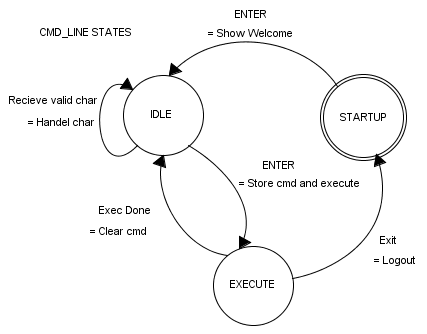
\includegraphics[width=.6\textwidth]{billeder/cmd_states.png}
	\caption{State diagram for shell task.}
	\label{fig:shell_task}
\end{figure}

Shell'en aktiveres, efter opnået forbindelse, ved at sende et \textbf{0x0D} \textit{(enter/return)}, hvorefter velkomstskærmen vises.
Der er et lille udvalg af kommandoer tilgængeligt for brugeren til at styre equalizeren - se tabel \ref{tab:shell_cmd} 

\begin{table}[h!]
	\caption{Kommando liste i EQ-ONE shell}
	\label{tab:shell_cmd}
	\begin{threeparttable}
		\begin{tabular}{l p{0.7\textwidth}}
			\toprule
			\textbf{Kommando}      & \textbf{Beskrivelse}   \\ 
			\midrule
			help		& Viser de tilgængelige kommandoer. \\
			eq       	& Skifter imellem tændt og slukket for equalizeren. \\
			eqon / eqoff & Tænder / slukker for equalizeren. \tnote{a}\\
			pN			& Skifter til profil nummer N = 1.. \\
			lp			& List tilgængelige profiler.\tnote{a}\\
			ps		    & Udskriv process oversigt. \\
			exit 		& Lukker shell'en ned. \\
			\bottomrule
		\end{tabular}
		
		\begin{tablenotes}
			\item[a] \textit{(ikke implementeret)}
		\end{tablenotes}
	\end{threeparttable}
\end{table}

Shell'en gør brug af ANSI/VT100 escape-sekvenserer, som fx. \textit{slet display} og \textit{set grafik modus}.
Derfor bør den terminalklient der anvendes understøtte dette, således at teksten bliver vist korrekt.







